\chapter{Theoretical framework}

\section{Phase-locked loop fundamentals}
\subsection{Basic structure}
\subsection{Key PLL parameters}
\subsubsection{Phase noise / jitter}
Jitter is defined as the time deviation ($\Delta_t$) of a signal's transition edges from their ideal positions in time. It is a metric of the outmost importance in the design of PLLs 
as it is a direct measure of the quality of the clock signal generated. Phase noise describes the same phenomenon in the frequency domain (the phase noise of a signal is the Fourier 
transform of the jitter) and is usually expressed in dBc/Hz.
\subsubsection{Output frequency}
It is defined as the range of frequencies that the PLL is capable of generating and can be determined by the VCO output range and the division ratio of the feedback frequency divider. This
is a key metric in establishing the application of the PLL (e.g., clock generation or RF synthesizer) and it bears significant importance in the design process due to the tradeoff 
it has with the phase noise performance of the PLL.
\subsubsection{Loop bandwidth}
The closed-loop bandwidth of a PLL is the frequency range over which the PLL can track the phase/frequency variations of the input signal (from DC to -3 dB from the open-loop 
gain). It affects the acquisition time and phase noise performance of the PLL.
\subsubsection{Noise bandwidth}
It is the PLL's noise due to the filter's loop bandwidth, the higher frequencies of the voltage-controlled oscillator (VCO) are the major
contributor to this effect, therefore the need to set a low enough bandwidth in order to supress the most out of it. Even if reducing the loop
bandwidth would be desirable to supress in-band phase noise, it's also necessary to take into consideration that there is a tradeoff between the
lock-in time and in-band phase noise.
\subsubsection{Beat-note period}
Defined as the time interval between successive "beats" (oscillations) observed at the phase detector output, in other words, is the inverse of
the frequency difference's magnitude between the reference and feedback signals as shown in figure \ref{fig:PFD_output}. Beat-note period is closely related to the acquisition time of the
PLL and can be estimated by equation \eqref{eq:T_beat}. This metric is a direct measure of the frequency mismatch between the reference and
the feedback signals.

\begin{equation}
    T_{beat} = \frac{1}{|f_{ref} - f_{feed}|}
    \label{eq:T_beat}
\end{equation}


\begin{minipage}{0.35\textwidth}
    \begin{center}
        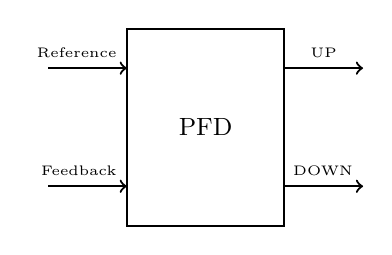
\begin{tikzpicture}
            \draw[->, thick] (-1,2) -- (0,2) node[anchor=south east] {\tiny Reference};
            \draw[->, thick] (-1, 0.5) -- (0,0.5) node[anchor=south east] {\tiny Feedback};
            \draw[thick] (0,0) rectangle (2,2.5);   %PFD
            \draw node at (1,1.25) {\small PFD};
            \draw[->, thick] (2,0.5) -- (3,0.5) node[anchor=south east] {\tiny DOWN};
            \draw[->, thick] (2,2) -- (3,2);
            \draw node at (2.5,2.2) {\tiny UP};
        \end{tikzpicture}
        \captionof{figure}{a) PFD block.}
        \label{fig:PFD_block}
    \end{center}
\end{minipage}
\hspace{0.13\textwidth}
\begin{minipage}{0.5\textwidth}
    \begin{center}
        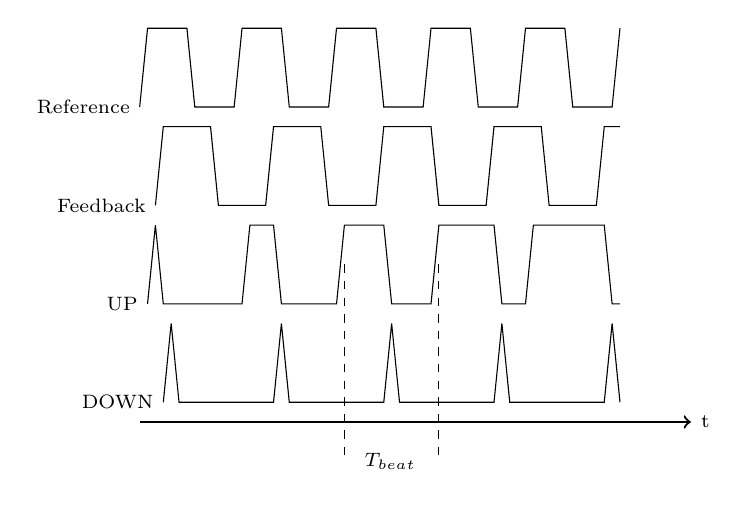
\begin{tikzpicture}
            \draw[->, thick] (0,1) -- (7,1) node[anchor=west] {\scriptsize t};
            \draw (0,5) node[anchor=east] {\scriptsize Reference} -- (0.1,6) -- (0.6,6) -- (0.7,5) -- (1.2,5) -- (1.3,6) -- (1.8,6) -- (1.9,5) -- (2.4,5) -- (2.5,6) -- (3,6) -- (3.1,5) -- (3.6,5) -- (3.7,6) -- (4.2,6) -- (4.3,5) -- (4.8,5) -- (4.9,6) -- (5.4,6) -- (5.5,5) -- (6,5) -- (6.1,6);
            \draw (0.2,3.75) node[anchor=east] {\scriptsize Feedback} -- (0.3,4.75) -- (0.9,4.75) -- (1,3.75) -- (1.6,3.75) -- (1.7,4.75) -- (2.3,4.75) -- (2.4,3.75) -- (3,3.75) -- (3.1,4.75) -- (3.7,4.75) -- (3.8,3.75) -- (4.4,3.75) -- (4.5,4.75) -- (5.1,4.75) -- (5.2,3.75) -- (5.8,3.75) -- (5.9,4.75) -- (6.1,4.75);
            \draw (0.1,2.5) node[anchor=east] {\scriptsize UP} -- (0.2,3.5) -- (0.3,2.5) -- (1.3,2.5) -- (1.4,3.5) -- (1.7,3.5) -- (1.8,2.5) -- (2.5,2.5) -- (2.6,3.5) -- (3.1,3.5) -- (3.2,2.5) -- (3.7,2.5) -- (3.8,3.5) -- (4.5,3.5) -- (4.6,2.5) -- (4.9,2.5) -- (5,3.5) -- (5.9,3.5) -- (6,2.5) -- (6.1,2.5);
            \draw (0.3,1.25) node[anchor=east] {\scriptsize DOWN} -- (0.4,2.25) -- (0.5,1.25) -- (1.7,1.25) -- (1.8,2.25) -- (1.9,1.25) -- (3.1,1.25) -- (3.2,2.25) -- (3.3,1.25) -- (4.5,1.25) -- (4.6,2.25) -- (4.7,1.25) -- (5.9,1.25) -- (6,2.25) -- (6.1,1.25);
            \draw[dashed] (2.6,3) -- (2.6,0.5) node[right, outer sep=4pt] {\scriptsize $T_{beat}$};
            \draw[dashed] (3.8,3) -- (3.8,0.5);
        \end{tikzpicture}
        \captionof{figure}{b) PFD output.}
        \label{fig:PFD_output}
    \end{center}
\end{minipage}
\subsubsection{Lock-in time}
Lock-in time (also called aquisition or settling time) is defined as the time for the PLL to lock on to the input reference phase and frequency within one 
beat-note period ($T_{beat}$) after a frequency change or startup of the system. This parameter measures the time required for the PLL
to achieve the final phase lock once the VCO frequency is within the lock-in range. The lock-in time can be estimated with equation
\eqref{eq:lock-in_time}.

\begin{equation}
    T_{lock-in} = \frac{ln(\epsilon)}{\zeta \omega_{n}}
    \label{eq:lock-in_time}
\end{equation}

where:

\[\epsilon = \text{acceptable phase error}\]
\[\zeta = \text{damping factor}\]
\[\omega_{n} = \text{natural frequency}\]


\subsubsection{Pull-in time}
In contrast with the lock-in time, the pull-in time is the required amount of time for the PLL to initially aquire lock on to the 
reference signal from an arbitrary starting frequency (when the VCO's initial frequency is far from the target).
\subsubsection{Lock-in range}
The frequency range within which the PLL locks to the reference frequency in one $T_{beat}$. Once the feedback signal is in this 
range, the PLL will enter lock state within the next T$_{beat}$.
\subsubsection{Pull-in range}
Range of frequency within which the PLL can aquire lock on to the reference signal once the VCO has the correct frequency and several 
beat-note periods have passed.
\subsubsection{Pull-out range}
The maximum allowed frequency or phase abrupt change applied to the reference signal beyond which the PLL unlocks.
\subsubsection{Hold range}
This parameter establishes the maximun theoretical frequency range for an input reference beyond which the PLL never locks. Hold range
is bigger than both lock-in and pull-in ranges.
\subsubsection{SNR}
The signal to noise ratio is an appropiate way to measure the impact of noise on a circuit. It's often used in most figures
of merit (FOM) for making fair comparisons between PLLs.
\subsubsection{Power consumption}
An important parameter in measuring the performance of integrated circuits. Often used in most FOMs.
\subsubsection{Spurs}
Spurious tones are unwanted periodic signals that appear at the output spectrum of the PLL. Spurs are completely deterministic, thus they are distinct
from phase noise which is random and spreads across the spectrum of the signal.

\subsection{Analog phase-locked loop}
The principles of operation of the digital PLL stem from its analog counterpart, therefore this subsection describes the fundamental 
building blocks of the analog PLL as well as a simplified model of the system which allows the circuit designer to analyse its behaviour.

\subsubsection{Linearized model}
The PLL is a non-linear system, yet it can be approximated quite accurately in to the linear system of figure \ref{fig:PFD_block} if certain
assumptions are taken in to consideration. The first of this assumptions is that the phase error ($\phi_{e}$) must be small enough, 
meaning the PLL is near lock state. Another one is that the characteristic of the phase detector must be approximately linear and given
by \eqref{eq:PD_linear_equation}. Lastly, the VCO range of operation must be within its linear region like in figure 1313 and thus be 
described by \eqref{eq:VCO_linear_equation}.

\begin{center}
        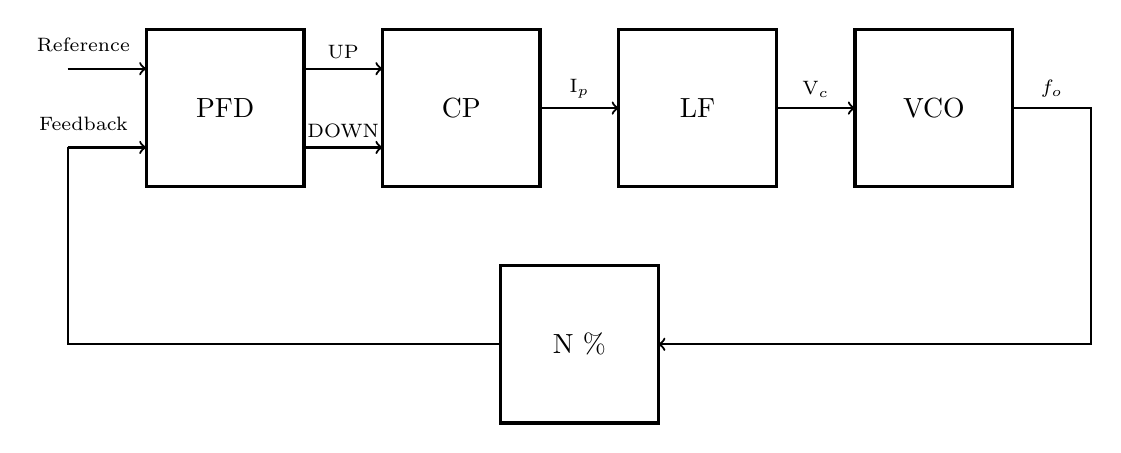
\begin{tikzpicture}
            [
                block/.style={rectangle, very thick, draw=black, minimum size=5pt}
            ]
            % PFD
            \draw[very thick] (0,3) rectangle (2,5);
            \draw node at (1,4) {PFD};
            \draw[->, thick] (2,4.5) -- node[above] {\scriptsize UP} (3,4.5);
            \draw[->, thick] (2,3.5) -- node[above] {\scriptsize DOWN} (3, 3.5);
            \draw[->, thick] (-1,4.5) -- (0,4.5);
            \draw[->, thick] (-1,3.5) -- (0, 3.5);
            \draw node at (-0.8,4.8) {\scriptsize Reference};
            \draw node at (-0.8,3.8) {\scriptsize Feedback};
            % CP
            \draw[very thick] (3,3) rectangle (5,5);
            \draw node at (4,4) {CP};
            \draw[->, thick] (5,4) -- node[above] {\scriptsize I$_{p}$} (6,4);
            % LF
            \draw[very thick] (6,3) rectangle (8,5);
            \draw node at (7,4) {LF};
            \draw[->, thick] (8,4) -- node[above] {\scriptsize V$_{c}$} (9,4);
            % VCO
            \draw[very thick] (9,3) rectangle (11,5);
            \draw node at (10,4) {VCO};
            \draw[->, thick] (11,4) -- node[above] {\scriptsize $f_{o}$} (12,4) -- (12,1) -- (6.5,1);
            % N %
            \draw[very thick] (4.5,0) rectangle (6.5,2);
            \draw node at (5.5,1) {N \%};
            \draw[thick] (4.5,1) -- (-1,1) -- (-1,3.5);
        \end{tikzpicture}
        \captionof{figure}{Block diagram of the linearized PLL model.}
        \label{fig:PLL_block_diagram}
\end{center}

% Poner figura de caracteristica de un VCO cross coupled pair

\begin{equation}
    v_{d} = K_{PD} \, \phi{e} + \underbrace{V_{do}}_{\text{\tiny free running voltage}}
    \label{eq:PD_linear_equation}
\end{equation}
\begin{equation}
    \Delta_{\omega_{o}} = K_{VCO} \, (V_{c} - V_{co})
    \label{eq:VCO_linear_equation}
\end{equation}

\noindent The closed-loop transfer function of the model shown in figure \ref{fig:PLL_block_diagram} can be obtained using Mason's gain equation \eqref{eq:Masons_rule}
in the system's equivalent of figure \ref{fig:PLL_block_diagram_TF}. Note that the loop filter is of second order.

\begin{equation}
    H(s) = \frac{\Sigma_{F.P} (1 - \Sigma_{not \, touching})}{1 - \Sigma_{loops}}
    \label{eq:Masons_rule}
\end{equation}

\begin{center}
    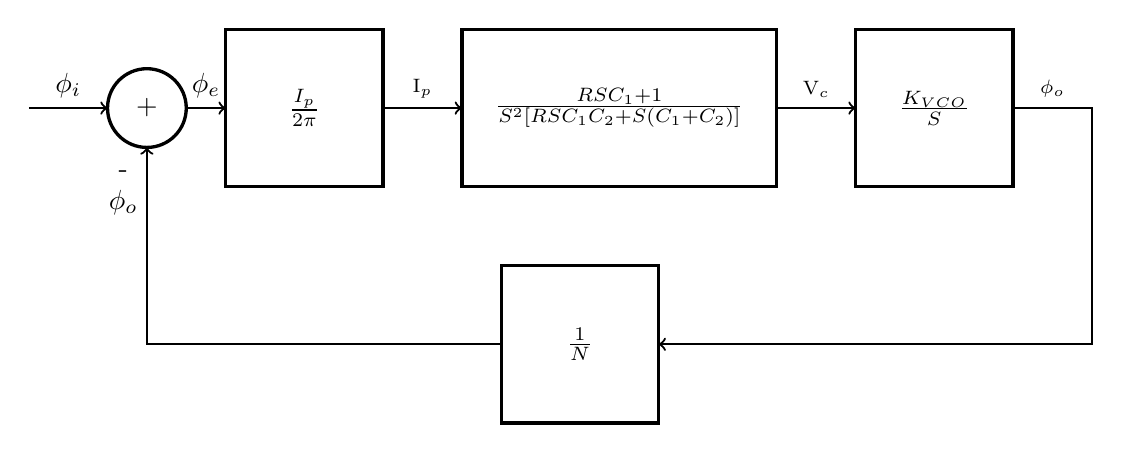
\begin{tikzpicture}
        [
            block/.style={rectangle, very thick, draw=black, minimum size=5pt}
        ]
        % PFD
        \draw[very thick] (0,4) circle (0.5);
        \draw node at (0,4) {+};
        \draw[->, thick] (0.5,4) -- node[above] {$\phi_{e}$} (1,4);
        \draw[->, thick] (-1.5,4) -- node[above] {$\phi_{i}$} (-0.5,4);
        \draw node at (-0.3,2.8) {$\phi_{o}$};
        \draw node at (-0.3,3.2) {-};
        % CP
        \draw[very thick] (1,3) rectangle (3,5);
        \draw node at (2,4) {$\frac{I_{p}}{2\pi}$};
        \draw[->, thick] (3,4) -- node[above] {\scriptsize I$_{p}$} (4,4);
        % LF
        \draw[very thick] (4,3) rectangle (8,5);
        \draw node at (6,4) {$\frac{RSC_{1} + 1}{S^2[RSC_{1}C_{2} + S(C_{1} + C_{2})]}$};
        \draw[->, thick] (8,4) -- node[above] {\scriptsize V$_{c}$} (9,4);
        % VCO
        \draw[very thick] (9,3) rectangle (11,5);
        \draw node at (10,4) {$\frac{K_{VCO}}{S}$};
        \draw[->, thick] (11,4) -- node[above] {\scriptsize $\phi_{o}$} (12,4) -- (12,1) -- (6.5,1);
        % N %
        \draw[very thick] (4.5,0) rectangle (6.5,2);
        \draw node at (5.5,1) {$\frac{1}{N}$};
        \draw[->, thick] (4.5,1) -- (0,1) -- (0,3.5);
    \end{tikzpicture}
    \captionof{figure}{Block diagram of the linearized PLL with each block transfer function.}
    \label{fig:PLL_block_diagram_TF}
\end{center}

\noindent Thus, the closed loop transfer function of this system is that of equation \eqref{eq:ACL}. This transfer function
describes the dynamics of the PLL entirely.

\begin{equation}
    A_{CL} = \frac{S I_{CP} R C_{1} K_{VCO} N \, + \, I_{CP} K_{VCO} N}{S^3 N R C_{1} C_{2} \, + \, S^2 N (C_{1} + C_{2}) \, + \, S I_{CP} R C_{1} \, + \, I_{CP} K_{VCO}}
    \label{eq:ACL}
\end{equation}
\subsubsection{Phase frequency detector}

A PLL that has a phase frequency detector (PFD) instead of a phase detector (PD) is superior because it can track changes in both
phase and frequency at the input signal. This approach provides robustness to the system because the PLL locks regardless of the initial
value of the output frequency, therefore making the pull-in range equal to the VCO tuning range.

\noindent The most common implementation of a PFD is shown in figure \ref{fig;PFD_schematic}. The operation of this circuit is as follows:
When either of the two signals arrive with a rising edge to the corresponding D flip-flop CLK terminal a HIGH state is pass along
to its output (Q), this result is mantained until the other signal's rising edge arrives at the other flip-flop because at that
moment in time the AND gate would activate and reset both flip-flops. This behavior can be observed in figure \ref{fig:PFD_transient_response}.

\begin{minipage}{0.49\textwidth}
    \begin{center}
        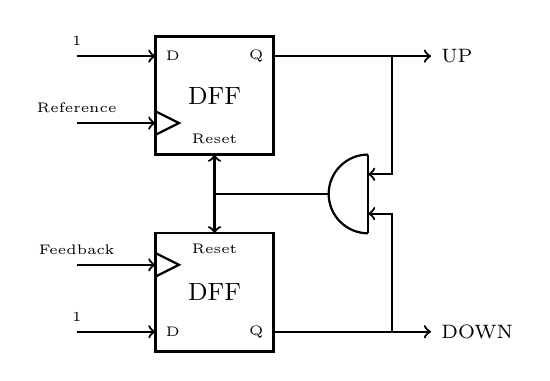
\begin{tikzpicture}
            \draw[thick] (0,0) rectangle (1.5,1.5);
            \draw[thick] (0,0.25) -- (0,0.55) -- (0.3,0.4) -- (0,0.25);
            \draw[->, thick] (-1,0.4) node[anchor=south] {\tiny Reference} -- (0,0.4);
            \draw node at (0.75,0.75) {\small DFF};
            \draw[->, thick] (-1,1.25) node[anchor=south] {\tiny 1} -- (0,1.25) node[anchor=west] {\tiny D};
            \draw[->, thick] (1.5,1.25) node[anchor=east] {\tiny Q} -- (3.5,1.25) node[right] {\scriptsize UP};
            \draw node at (0.75, 0.2) {\tiny Reset};
            
            \draw[thick] (0,-1) rectangle (1.5,-2.5);
            \draw[thick] (0,-1.25) -- (0,-1.55) -- (0.3,-1.4) -- (0,-1.25);
            \draw[->, thick] (-1,-1.4) node[anchor=south] {\tiny Feedback} -- (0,-1.4);
            \draw node at (0.75,-1.75) {\small DFF};
            \draw[->, thick] (-1,-2.25) node[anchor=south] {\tiny 1} -- (0,-2.25) node[anchor=west] {\tiny D};
            \draw[->, thick] (1.5,-2.25) node[anchor=east] {\tiny Q} -- (3.5,-2.25) node[anchor=west] {\scriptsize DOWN};
            \draw node at (0.75, -1.2) {\tiny Reset};
    
            \draw[->, thick] (3,1.25) -- (3,-0.25) -- (2.7,-0.25);
            \draw[->, thick] (3,-2.25) -- (3,-0.75) -- (2.7,-0.75);
            \draw[thick] (2.7,0) -- (2.7,-1);
            \draw[thick] (2.7,0) arc (90:270:0.5);
            \draw[->, thick] (2.2,-0.5) -- (0.75,-0.5) -- (0.75,0);
            \draw[->, thick] (0.75,-0.5) -- (0.75,-1);
        \end{tikzpicture}
        \captionof{figure}{Three states PFD implementation.}
        \label{fig;PFD_schematic}
    \end{center}
\end{minipage}
\begin{minipage}{0.49\textwidth}
    \begin{center}
        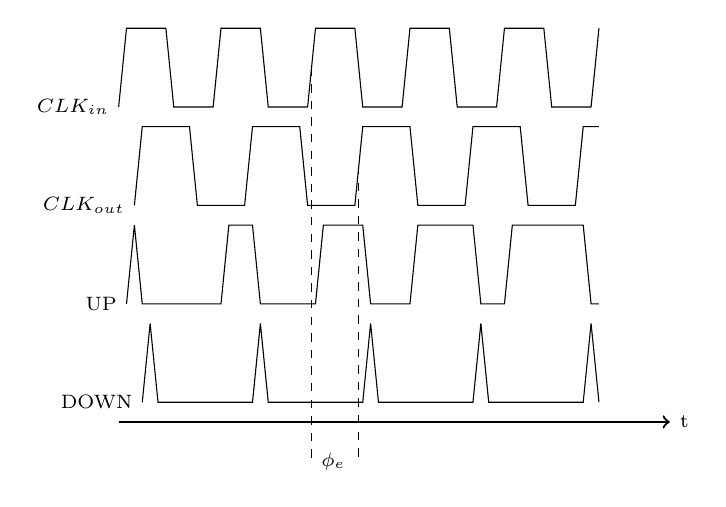
\begin{tikzpicture}
            \draw[->, thick] (0,1) -- (7,1) node[anchor=west] {\scriptsize t};
            \draw (0,5) node[anchor=east] {\scriptsize $CLK_{in}$} -- (0.1,6) -- (0.6,6) -- (0.7,5) -- (1.2,5) -- (1.3,6) -- (1.8,6) -- (1.9,5) -- (2.4,5) -- (2.5,6) -- (3,6) -- (3.1,5) -- (3.6,5) -- (3.7,6) -- (4.2,6) -- (4.3,5) -- (4.8,5) -- (4.9,6) -- (5.4,6) -- (5.5,5) -- (6,5) -- (6.1,6);
            \draw (0.2,3.75) node[anchor=east] {\scriptsize $CLK_{out}$} -- (0.3,4.75) -- (0.9,4.75) -- (1,3.75) -- (1.6,3.75) -- (1.7,4.75) -- (2.3,4.75) -- (2.4,3.75) -- (3,3.75) -- (3.1,4.75) -- (3.7,4.75) -- (3.8,3.75) -- (4.4,3.75) -- (4.5,4.75) -- (5.1,4.75) -- (5.2,3.75) -- (5.8,3.75) -- (5.9,4.75) -- (6.1,4.75);
            \draw (0.1,2.5) node[anchor=east] {\scriptsize UP} -- (0.2,3.5) -- (0.3,2.5) -- (1.3,2.5) -- (1.4,3.5) -- (1.7,3.5) -- (1.8,2.5) -- (2.5,2.5) -- (2.6,3.5) -- (3.1,3.5) -- (3.2,2.5) -- (3.7,2.5) -- (3.8,3.5) -- (4.5,3.5) -- (4.6,2.5) -- (4.9,2.5) -- (5,3.5) -- (5.9,3.5) -- (6,2.5) -- (6.1,2.5);
            \draw (0.3,1.25) node[anchor=east] {\scriptsize DOWN} -- (0.4,2.25) -- (0.5,1.25) -- (1.7,1.25) -- (1.8,2.25) -- (1.9,1.25) -- (3.1,1.25) -- (3.2,2.25) -- (3.3,1.25) -- (4.5,1.25) -- (4.6,2.25) -- (4.7,1.25) -- (5.9,1.25) -- (6,2.25) -- (6.1,1.25);
            \draw[dashed] (2.45,5.5) -- (2.45,0.5) node[anchor=west] {\scriptsize $\phi_{e}$};
            \draw[dashed] (3.05,4.25) -- (3.05,0.5);
        \end{tikzpicture}
        \captionof{figure}{Transient response of the PFD.}
        \label{fig:PFD_transient_response}
    \end{center}
\end{minipage}

\subsubsection{Charge pump}

\subsubsection{Loop filter}
\subsubsection{Voltage-controlled oscillator}

\subsubsection{Frequency divider}

\section{Digital phase-locked loop}
anan
\section{Time-to-digital converter}
\subsection{Delay-locked loop fundamentals}
\subsection{TDC as a phase detector}

\section{65 nm CMOS technology}
